\documentclass[border=4pt,12pt]{standalone}
% House style for redrawn exam diagrams (diagram-v4: 0.4pt lines, filled -latex arrows, fine dashes; stipple and hatching drawn as real dots/lines (no PDF/SVG patterns, so they render in every browser and at any scale); transparent background). Every figure \input's this.
\usepackage{amsmath,amssymb}
\usepackage{txfonts}
\usepackage{pdfrender,xcolor}
% \halo{text}: label on shading. The shading stops just around each letter's outline (a thin knock-out that follows the
% glyphs, like the papers' typesetting), never a box. Owner: "I don't want a box around the text".
\newcommand{\halo}[1]{\leavevmode\rlap{\pdfrender{TextRenderingMode=2,LineWidth=2.2pt,LineJoinStyle=1,StrokeColor=white,FillColor=white}#1}#1}
\usepackage{tikz,pgfplots}
\pgfplotsset{compat=1.18}
\usetikzlibrary{arrows.meta,calc,angles,quotes,patterns,patterns.meta,intersections,positioning,decorations.markings,shapes.geometric}
% Stipple and hatching are drawn as actual dots / lines clipped to the region (path picture), NOT as pattern fills:
% SVG <pattern> fills vanish or blur when browsers scale the image, so the owner could not see the shading.
% Each dot is a 0.72pt square (keeps SVGs small; reads as a dot at print size). Dots sit on one global staggered grid, so neighbouring regions line up.
\makeatletter
\newdimen\ex@x \newdimen\ex@y \newdimen\ex@xa \newdimen\ex@ya \newdimen\ex@xb \newdimen\ex@yb \newcount\ex@row
\def\exam@stipplecolor{black!75}\def\exam@dotr{0.42pt}\def\exam@dotgap{2.5}
\def\ex@rowdots{\ifdim\ex@x<\ex@xb \pgfpathrectangle{\pgfqpoint{\dimexpr\ex@x-0.36pt\relax}{\dimexpr\ex@y-0.36pt\relax}}{\pgfqpoint{0.72pt}{0.72pt}}\advance\ex@x by \exam@dotgap pt\relax\expandafter\ex@rowdots\fi}
\def\exam@stipple{%
  \pgftransformreset% dots are sized in real points even inside scaled pictures
  \pgfpointanchor{path picture bounding box}{south west}\ex@xa=\pgf@x \ex@ya=\pgf@y
  \pgfpointanchor{path picture bounding box}{north east}\ex@xb=\pgf@x \ex@yb=\pgf@y
  \pgfsetfillcolor{\exam@stipplecolor}\pgfmathsetmacro\ex@h{\exam@dotgap/2}%
  \pgfmathtruncatemacro\ex@r{floor(\ex@ya/\ex@h)-1}\ex@row=\ex@r\relax
  \ex@y=\ex@r\dimexpr\ex@h pt\relax
  \loop\ifdim\ex@y<\ex@yb
    \pgfmathtruncatemacro\ex@c{floor(\ex@xa/\exam@dotgap)-1}\ex@x=\ex@c\dimexpr\exam@dotgap pt\relax
    \ifodd\ex@row \advance\ex@x by \ex@h pt\fi
    \ex@rowdots
    \advance\ex@y by \ex@h pt \advance\ex@row by 1
    \ifnum\numexpr\ex@row-(\ex@row/4)*4\relax=0 \pgfusepath{fill}\fi% flush every 4 rows: bounded TeX memory, few clip copies in the SVG
  \repeat\pgfusepath{fill}}
\newdimen\ex@d
\def\exam@hatch#1{% #1 = 1 for /, -1 for \ ; lines 45 degrees, 3pt apart
  \pgftransformreset
  \pgfpointanchor{path picture bounding box}{south west}\ex@xa=\pgf@x \ex@ya=\pgf@y
  \pgfpointanchor{path picture bounding box}{north east}\ex@xb=\pgf@x \ex@yb=\pgf@y
  \ex@d=\dimexpr\ex@yb-\ex@ya\relax \ex@x=\dimexpr\ex@xa-\ex@d\relax
  \loop\ifdim\ex@x<\ex@xb
    \ifnum#1>0 \pgfpathmoveto{\pgfqpoint{\ex@x}{\ex@ya}}\pgfpathlineto{\pgfqpoint{\dimexpr\ex@x+\ex@d\relax}{\ex@yb}}%
    \else \pgfpathmoveto{\pgfqpoint{\ex@x}{\ex@yb}}\pgfpathlineto{\pgfqpoint{\dimexpr\ex@x+\ex@d\relax}{\ex@ya}}\fi
    \advance\ex@x by 4.24pt
  \repeat
  \pgfsetlinewidth{0.4pt}\pgfsetstrokecolor{black}\pgfusepath{stroke}}
\def\examstipple{\exam@stipple}\def\examhatch{\exam@hatch}\def\examsetstipplecolor#1{\def\exam@stipplecolor{#1}}\def\examsetdotgap#1{\def\exam@dotgap{#1}}
\makeatother
% (legacy pattern kept for old files)
% staggered stipple like the NESA papers' dotted shading
\pgfdeclarepatternformonly{exam stipple}{\pgfpointorigin}{\pgfqpoint{2.2pt}{2.2pt}}{\pgfqpoint{2.2pt}{2.2pt}}{%
  \pgfpathcircle{\pgfqpoint{0.55pt}{0.55pt}}{0.42pt}\pgfpathcircle{\pgfqpoint{1.65pt}{1.65pt}}{0.42pt}\pgfusepath{fill}}
\tikzset{
  every picture/.style={line width=0.6pt, >={Latex[length=2mm,width=1.3mm]}},
  curve/.style={line width=0.6pt},
  open arrow/.style={-{Latex[length=2mm,width=1.3mm]}},  % owner: filled -latex heads everywhere, no open chevrons
  aux/.style={dash pattern=on 2pt off 1.5pt, line width=0.6pt},
  shade/.code={\def\exA{#1}\def\exB{none}\ifx\exA\exB\else\pgfkeysalso{fill=black!18}\fi},
  shade/.default=on,
  shade dots/.style={fill=none, path picture={\examstipple}},
  stipple color/.code={\examsetstipplecolor{#1}},
  stipple gap/.code={\examsetdotgap{#1}},
  shade dense dots/.style={fill=none, stipple gap=1.6, path picture={\examstipple}},
  shade hatch/.style={fill=none, path picture={\examhatch{1}}},
  shade hatch reverse/.style={fill=none, path picture={\examhatch{-1}}},
  shade solid/.style={fill=black},
  pt/.style={circle, fill, inner sep=1.1pt},
  open pt/.style={circle, draw, fill=white, inner sep=1.1pt},
}
\pgfplotsset{
  exam axes/.style={axis lines=middle, axis line style={->}, xlabel={$x$}, ylabel={$y$},
    xlabel style={anchor=west}, ylabel style={anchor=south}, tick label style={font=\small},
    every axis plot/.append style={line width=0.6pt, black}, samples=200, clip=false,
    enlargelimits=false, axis on top},
}

\begin{document}
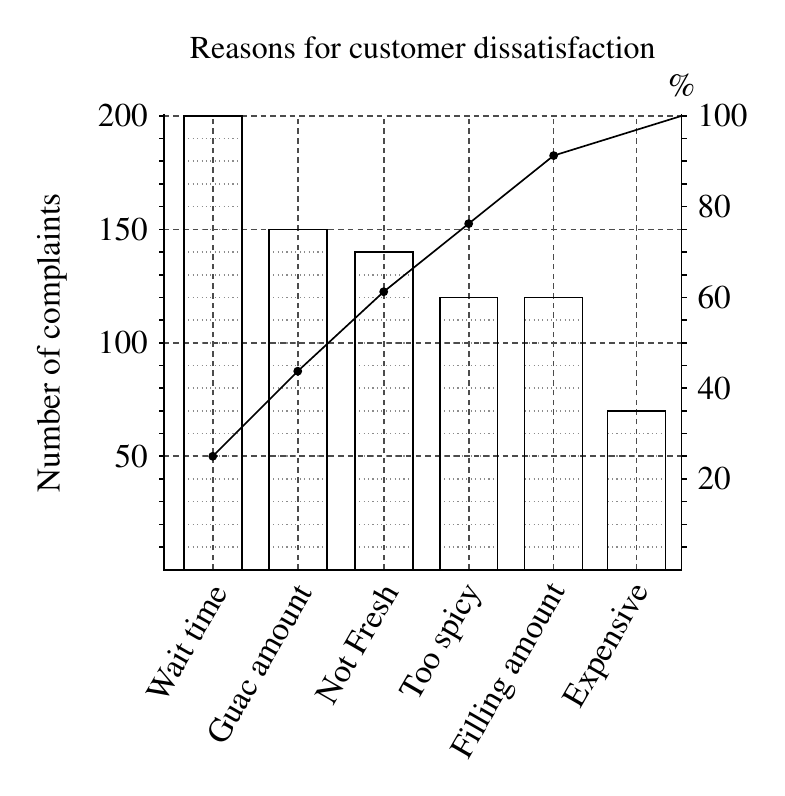
\begin{tikzpicture}[x=0.0127cm,y=-0.0127cm,font=\fontsize{12}{14}\selectfont]
  \begin{scope}\clip (142,557) rectangle (200,103.0);
    \foreach \v in {10,20,...,190} \draw[black!45,dash pattern=on 0.4pt off 1.2pt] (142,557-2.27*\v) -- (200,557-2.27*\v);\end{scope}
  \begin{scope}\clip (227,557) rectangle (285,216.5);
    \foreach \v in {10,20,...,190} \draw[black!45,dash pattern=on 0.4pt off 1.2pt] (227,557-2.27*\v) -- (285,557-2.27*\v);\end{scope}
  \begin{scope}\clip (313,557) rectangle (371,239.2);
    \foreach \v in {10,20,...,190} \draw[black!45,dash pattern=on 0.4pt off 1.2pt] (313,557-2.27*\v) -- (371,557-2.27*\v);\end{scope}
  \begin{scope}\clip (398,557) rectangle (456,284.6);
    \foreach \v in {10,20,...,190} \draw[black!45,dash pattern=on 0.4pt off 1.2pt] (398,557-2.27*\v) -- (456,557-2.27*\v);\end{scope}
  \begin{scope}\clip (483,557) rectangle (541,284.6);
    \foreach \v in {10,20,...,190} \draw[black!45,dash pattern=on 0.4pt off 1.2pt] (483,557-2.27*\v) -- (541,557-2.27*\v);\end{scope}
  \begin{scope}\clip (566,557) rectangle (624,398.1);
    \foreach \v in {10,20,...,190} \draw[black!45,dash pattern=on 0.4pt off 1.2pt] (566,557-2.27*\v) -- (624,557-2.27*\v);\end{scope}
  \draw[black!70,dash pattern=on 2pt off 1.5pt] (122,443.5) -- (640,443.5);
  \draw[black!70,dash pattern=on 2pt off 1.5pt] (122,330.0) -- (640,330.0);
  \draw[black!70,dash pattern=on 2pt off 1.5pt] (122,216.5) -- (640,216.5);
  \draw[black!70,dash pattern=on 2pt off 1.5pt] (122,103.0) -- (640,103.0);
  \draw[black!70,dash pattern=on 2pt off 1.5pt] (171,557) -- (171,103.0);
  \draw[black!70,dash pattern=on 2pt off 1.5pt] (256,557) -- (256,103.0);
  \draw[black!70,dash pattern=on 2pt off 1.5pt] (342,557) -- (342,103.0);
  \draw[black!70,dash pattern=on 2pt off 1.5pt] (427,557) -- (427,103.0);
  \draw[black!70,dash pattern=on 2pt off 1.5pt] (512,557) -- (512,103.0);
  \draw[black!70,dash pattern=on 2pt off 1.5pt] (595,557) -- (595,103.0);
  \draw (142,557) rectangle (200,103.0);
  \draw (227,557) rectangle (285,216.5);
  \draw (313,557) rectangle (371,239.2);
  \draw (398,557) rectangle (456,284.6);
  \draw (483,557) rectangle (541,284.6);
  \draw (566,557) rectangle (624,398.1);
  \draw (122,101.0) -- (122,557) -- (640,557) -- (640,101.0);
  \foreach \v in {10,20,...,200} \draw (122,557-2.27*\v) -- (117,557-2.27*\v);
  \foreach \p in {5,10,...,100} \draw (640,557-4.54*\p) -- (645,557-4.54*\p);
  \node[anchor=east] at (116,443.5) {50};
  \node[anchor=east] at (116,330.0) {100};
  \node[anchor=east] at (116,216.5) {150};
  \node[anchor=east] at (116,103.0) {200};
  \node[anchor=west] at (646,466.2) {20};
  \node[anchor=west] at (646,375.4) {40};
  \node[anchor=west] at (646,284.6) {60};
  \node[anchor=west] at (646,193.8) {80};
  \node[anchor=west] at (646,103.0) {100};
  \node at (640,73) {\%};
  \node[rotate=90] at (10,330.0) {Number of complaints};
  \node[font=\fontsize{11.5}{14}\selectfont] at (381.0,35) {Reasons for customer dissatisfaction};
  \node[rotate=60,anchor=east,inner sep=1pt] at (179,571) {Wait time};
  \node[rotate=60,anchor=east,inner sep=1pt] at (264,571) {Guac amount};
  \node[rotate=60,anchor=east,inner sep=1pt] at (350,571) {Not Fresh};
  \node[rotate=60,anchor=east,inner sep=1pt] at (435,571) {Too spicy};
  \node[rotate=60,anchor=east,inner sep=1pt] at (520,571) {Filling amount};
  \node[rotate=60,anchor=east,inner sep=1pt] at (603,571) {Expensive};
  \draw (171,443.5) -- (256,358.4) -- (342,278.9) -- (427,210.8) -- (512,142.7) -- (640,103.0);
  \fill (171,443.5) circle (1.6pt);
  \fill (256,358.4) circle (1.6pt);
  \fill (342,278.9) circle (1.6pt);
  \fill (427,210.8) circle (1.6pt);
  \fill (512,142.7) circle (1.6pt);
\end{tikzpicture}
\end{document}
